\documentclass[a4paper, fontsize = 8pt, landscape]{scrartcl}
\usepackage{../../../misc_files/LateX/layout_and_colours}
\makeatletter
\def\input@path{{content/lecture_summary/}{content/examples/}}
\makeatother
\graphicspath{{content/images/}{content/lecture_summary/images/}{content/examples/images/}}

\title{Höhere Mathematik 2}
\author{Jil Zerndt}
\date{FS 2025}

\createtitlepagestyle
\createmainpagestyle
\begin{document}
\begin{multicols}{3}
	\thispagestyle{TitlePageStyle}
	\maketitle
	\sffamily
	\section{Numerische Lösung nicht linearer Gleichungssysteme}

\begin{remark}
    LGS = lineares Gleichungssystem, NGS = nichtlineares Gleichungssystem
\end{remark}



\raggedcolumns

\begin{definition}{Skalarwertige Funktionen}
    $f: D \subset \R^n \to W \subset \R$
    \vspace{-2mm}
    $$(x_1, x_2, \ldots, x_n) \mapsto y = f(x_1, x_2, \ldots, x_n)$$
    \small
    $f$ mit $n$ unabhängigen Variablen $x_1, \ldots, x_n$ und einer abhängigen Variablen $y$,
    die jedem $(x_1, x_2, \ldots, x_n)$ aus Definitionsmenge $D \subset \R^n$ genau ein $y \in W \subset \R$ zuordnet.
    Ergebnis: $y \in \R$ = Skalar (eine Zahl) 
\end{definition}

\begin{concept}{Vektorwertige Funktion} gibt einen \textbf{Vektor} zurück (statt Skalar)\\
    Sei $\textbf{f}: \R^n \to \R^m$ eine Funktion mit $n$ Variablen.
    \vspace{-2mm}
    $$\textbf{f}(x_1 \ldots, x_n) = \begin{psmallmatrix} y_1 = f_1(x_1, x_2, \ldots, x_n) \\ y_2 = f_2(x_1, x_2, \ldots, x_n) \\ ... \\ y_m = f_m(x_1, x_2, \ldots, x_n) \end{psmallmatrix}$$
    \small wobei die $m$ Komponenten $f_i: \R^n \to \R$ für $i = 1, 2, \ldots, n$ von $\textbf{f}$ wieder \textbf{skalarwertige} Funktionen sind.
\end{concept}

\begin{theorem}{Nichtlineares Gleichungssystem (NGS)}\\
    Lösungen des NGS sind Nullstellen der Funktion:
    \vspace{-2mm}
    $$\textbf{f}: \R^2 \to \R^2 \quad \textbf{f}(x) = \begin{psmallmatrix} f_1 (x_1, x_2) \\ f_2 (x_1, x_2) \end{psmallmatrix} = \begin{psmallmatrix} 0\\ 0 \end{psmallmatrix}$$
    \small
    Ein solches System lässt sich nicht in die Form $Ax = b$ bringen. \\
    Geometrisch lassen sich die Lösungen als Schnittpunkte der beiden Funktionen interpretieren.
\end{theorem}

\begin{corollary}{Lineare Funktionen von LGS}
    $$\textbf{A} \overrightarrow{\textbf{x}} = \overrightarrow{\textbf{b}} \Rightarrow \underbrace{\textbf{A} \overrightarrow{\textbf{x}} - \overrightarrow{\textbf{b}} = \overrightarrow{\textbf{0}}}_{\overrightarrow{\textbf{f}}(\overrightarrow{\textbf{x}})} \Rightarrow \overrightarrow{\textbf{f}}(x_1, x_2, x_3) = 0 \begin{psmallmatrix} x_1 \\ x_2 \\ x_3 \end{psmallmatrix} = \begin{psmallmatrix} 0 \\ 0 \\ 0 \end{psmallmatrix}$$
    \resizebox{\textwidth}{!}{
    $\overrightarrow{\textbf{f}}(\overrightarrow{\textbf{x}}) = \textbf{A} \overrightarrow{\textbf{x}} - \overrightarrow{\textbf{b}} = \begin{psmallmatrix} 4 & -1 & 1 \\ -2 & 5 & 1 \\ 1 & -2 & 5 \end{psmallmatrix} \begin{psmallmatrix} x_1 \\ x_2 \\ x_3 \end{psmallmatrix} - \begin{psmallmatrix} 5 \\ 11 \\ 12 \end{psmallmatrix}, \quad
    \textbf{f}(x_1, x_2, x_3) = \begin{psmallmatrix} f_1 = 4x_1 - x_2 + x_3 - 5 \\ f_2 = -2x_1 + 5x_2 + x_3 - 11 \\ f_3 = x_1 - 2x_2 + 5x_3 - 12 \end{psmallmatrix}$}
\end{corollary}


\begin{concept}{Analytische Darstellung}
    \begin{itemize}
        \item \textbf{Explizite Darstellung:} $y = f(x_1, \ldots, x_n)$
        \item \textbf{Implizite Darstellung:} $F(x, y) = 0$
        \item \textbf{Parameterdarstellung:} $x = x(t), y = y(t)$
    \end{itemize}
\end{concept}

\begin{concept}{Darstellung durch Wertetabelle}
    Sei $f: \R^n \to \R^m$ eine Funktion.\\
    In $z = f(x,y)$ Werte von $x$ und $y$ einsetzen (der Reihe nach): \\
    $$\begin{psmallmatrix} z_{11} & z_{12} & \ldots & z_{1m} \\ z_{m1} & z_{m2} & \ldots & z_{mn} \end{psmallmatrix} \quad\quad\quad\quad\quad\quad\quad\quad\quad\quad\quad\quad\quad\quad.$$
\end{concept}

\begin{minipage}{0.5\linewidth}
\begin{concept}{Funktion als Fläche im Raum}\\
    $f$ ordnet jedem Punkt $(x, y) \in D$ in Ebene Wert $z=f(x, y)$ zu \\($\rightarrow$ Höhenkoordinate)    
\end{concept}

\begin{concept}{Schnittkurvendiagramm}\\
    Fläche $z=f(x, y)$ bei konstanten Höhe $z$ schneiden: Schnittkurve. 
    Diese in $(x, y)$-Ebene projizieren: Höhenlinie.
\end{concept}
\end{minipage}
\begin{minipage}{0.5\linewidth}
\vspace{-8mm}
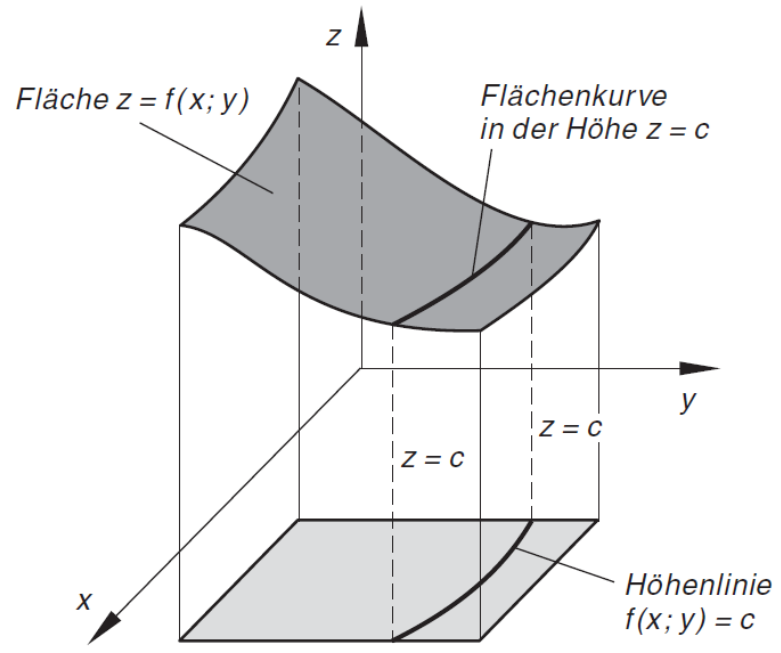
\includegraphics[width=\linewidth]{grafische_darstellung_detailed.png}
\small hellgraue Fläche = Definitionsbereich D
\end{minipage}

\subsubsection{Partielle Ableitungen}

\begin{theorem}{Partielle Ableitung}
$
f^{\prime}(x_0)=\lim _{\Delta x \rightarrow 0} \frac{(f(x_0+\Delta x)-f(x_0))}{\Delta x}
$
$$\text{Ableitung nach x: } f_x=\frac{\partial f}{\partial x}(x, y)=\lim _{\Delta x \rightarrow 0} \frac{f(x+\Delta x, y)-f(x, y)}{\Delta x}$$
$$\text{Ableitung nach y: } f_y=\frac{\partial f}{\partial y}(x, y)=\lim _{\Delta y \rightarrow 0} \frac{f(x, y+\Delta y)-f(x, y)}{\Delta y}$$
\end{theorem}



\begin{KR}{Partielle Ableitungen berechnen}
    \small
    \begin{enumerate}
        \item Variable identifizieren: nach welcher Variable ableiten?
        \item Alle anderen Variablen während Ableitung nur Konstanten
        \item Standardableitungsregeln anwenden und Ergebnis korrekt notieren
    \end{enumerate}
\end{KR}

\begin{definition}{Jacobi-Matrix}
    \resizebox{0.7\textwidth}{!}{
$f: \mathbb{R}^n \rightarrow \mathbb{R}^m$ mit $y = f(x)$ und $x = (x_1, x_2, ..., x_n)^T \in \mathbb{R}^n$}

Jacobi-Matrix enthält alle partiellen Ableitungen 1. Ordnung von $f$:
\vspace{-2mm}\\
$$f(x) = \begin{psmallmatrix}
    y_1=f_1(x) \\
    y_2=f_2(x) \\
    ...\\
    y_m=f_m(x)
\end{psmallmatrix} \rightarrow 
Df(x) := \begin{bsmallmatrix}
\frac{\partial f_1}{\partial x_1}(x) & \frac{\partial f_1}{\partial x_2}(x) & \cdots & \frac{\partial f_1}{\partial x_n}(x) \\
\frac{\partial f_2}{\partial x_1}(x) & \frac{\partial f_2}{\partial x_2}(x) & \cdots & \frac{\partial f_2}{\partial x_n}(x) \\
\cdots & \cdots & \cdots & \cdots \\
\frac{\partial f_m}{\partial x_1}(x) & \frac{\partial f_m}{\partial x_2}(x) & \cdots & \frac{\partial f_m}{\partial x_n}(x)
\end{bsmallmatrix}$$
\end{definition}

\begin{concept}{Linearisierung}
Die verallgemeinerte \textcolor{purple}{\textbf{Tangentengleichung}}
$$g(x) = f(x^{(0)}) + Df(x^{(0)}) \cdot (x - x^{(0)})$$ 
\small
beschreibt lineare Funktion, $f(x) \approx g(x)$ in Umgebung von $x^{(0)}=(x_1^{(0)}, x_2^{(0)}, \ldots, x_n^{(0)})^T \in \mathbb{R}^n$. 
Man spricht von der \textbf{Linearisierung} der Funktion $y = f(x)$ in einer Umgebung von $x^{(0)}$ ($x^{(k)}$ bezeichnet Vektor aus $\R^n$ nach $k$-ter Iteration).
\end{concept}

\begin{corollary}{Tangentialebene}
    \resizebox{0.7\textwidth}{!}{
    $f: \mathbb{R}^2 \longrightarrow \mathbb{R}$, $y=f(x_1, x_2)$, $\boldsymbol{x}^{(0)}=(x_1^{(0)}, x_2^{(0)})^T \in \mathbb{R}^2$ }

    Spezielle Jacobi-Matrix (nur ein Zeilenvektor mit zwei Elementen):
    \vspace{-2mm}\\
    $$Df(x^{(0)}) = \left(\frac{\partial f}{\partial x_1}(x_1^{(0)}, x_2^{(0)}), \frac{\partial f}{\partial x_2}(x_1^{(0)}, x_2^{(0)})\right)$$
    Linearisierung $g(x_1, x_2)$ die Gleichung der Tangentialebene: 
    $$=f(x_1^{(0)}, x_2^{(0)}) + (\frac{\partial f}{\partial x_1}(x_1^{(0)}, x_2^{(0)}), \frac{\partial f}{\partial x_2}(x_1^{(0)}, x_2^{(0)})) \cdot \binom{x_1 - x_1^{(0)}}{x_2 - x_2^{(0)}}$$
    $$= f(x_1^{(0)}, x_2^{(0)}) + \frac{\partial f}{\partial x_1}(x_1^{(0)}, x_2^{(0)}) \cdot (x_1 - x_1^{(0)}) + \frac{\partial f}{\partial x_2}(x_1^{(0)}, x_2^{(0)}) \cdot (x_2 - x_2^{(0)})$$
    \small
    Sie enthält sämtliche im Flächenpunkt 
    $\stackrel{\bullet}{P}=(x_1^{(0)}, x_2^{(0)}, f(x_1^{(0)}, x_2^{(0)}))$ \\
    an die Bildfläche von $y=f(x_1, x_2)$ angelegten Tangenten.
\end{corollary}

\begin{KR}{Jacobi-Matrix berechnen und linearisieren}\\
Sei $f: \mathbb{R}^n \rightarrow \mathbb{R}^m$ mit $y = f(x)$ und $x = (x_1, x_2, ..., x_n)^T \in \mathbb{R}^n$. 
\vspace{-2mm}\\
\begin{enumerate}
    \item Identifiziere die Komponentenfunktionen $f_1, f_2, ..., f_m$ und \\ Variablen $x_1, x_2, ..., x_n$.
    \item Berechne partielle Ableitungen $\frac{\partial f_i}{\partial x_j}$ für $i = 1, ..., m$, $j = 1, ..., n$.
    \item Stelle die Jacobi-Matrix $Df(x)$ auf
    \item Werte Jacobi-Matrix an Entwicklungspunkt $x^{(0)}$ aus\\ (Werte für $x_1, x_2, ..., x_n$ einsetzen)
    \item Berechne Linearisierung $g(x)$ mit Tangentengleichung
\end{enumerate}
\end{KR}

\begin{remark}
    Struggle $\in \R$
\end{remark}

\begin{example2}{Jacobi-Matrix und Linearisierung} \small
$f(x, y, z) = \begin{psmallmatrix} e^{xy} + z^2 - 3 \\ \sin(x + y) - z \\ x^2 + y^2 + z^2 - 6 \end{psmallmatrix}$

\textbf{Jacobi-Matrix:}
$Df(x, y, z) = \begin{bsmallmatrix} ye^{xy} & xe^{xy} & 2z \\ \cos(x + y) & \cos(x + y) & -1 \\ 2x & 2y & 2z \end{bsmallmatrix}$

\textbf{Linearisierung an $(1, 0, 1)^T$:}

\resizebox{\textwidth}{!}{
$f(1, 0, 1) = \begin{psmallmatrix} e^0 + 1 - 3 \\ \sin(1) - 1 \\ 1 + 0 + 1 - 6 \end{psmallmatrix} = \begin{psmallmatrix} -1 \\ \sin(1) - 1 \\ -4 \end{psmallmatrix}, \quad
Df(1, 0, 1) = \begin{bsmallmatrix} 0 & 1 & 2 \\ \cos(1) & \cos(1) & -1 \\ 2 & 0 & 2 \end{bsmallmatrix}$}

Linearisierung: $g(x, y, z) = f(1, 0, 1) + Df(1, 0, 1) \cdot \begin{psmallmatrix} x - 1 \\ y - 0 \\ z - 1 \end{psmallmatrix}$

$$g(x, y, z) = \begin{psmallmatrix} -1 + y + 2(z-1) \\ \sin(1) - 1 + \cos(1)(x-1) + \cos(1)y - (z-1) \\ -4 + 2(x-1) + 2(z-1) \end{psmallmatrix}$$

\textbf{Geometrische Bedeutung:}
Linearisierung approximiert nichtlineare Funktion $f$ nahe des Punktes $(1, 0, 1)^T$ durch lineare Funktion. Entspricht der Tangentialebene an die durch $f = 0$ definierte Fläche im 3D Raum.
\end{example2}

\raggedcolumns

\subsubsection{Nullstellenbestimmung für NGS}

\begin{definition}{Problemstellung zur Nullstellenbestimmung}\\
Gegeben: $n \in \mathbb{N}$, $f: \mathbb{R}^n \rightarrow \mathbb{R}^n$ Gesucht: Vektor $\bar{x} \in \mathbb{R}^n$ mit $f(\bar{x}) = 0$

Komponentenweise: Gegeben: $n$ Funktionen $f_i: \mathbb{R}^n \rightarrow \mathbb{R}$ (Komponenten von $f$) Gesucht: Vektor $\bar{x} \in \mathbb{R}^n$ mit $f_i(\bar{x}) = 0$ für $i = 1, ..., n$.
\end{definition}

\begin{KR}{Newton-Verfahren für NGS} \small{(Quadratische Konv.)}\\
    \normalsize
    Gesucht: Nullstellen von $f: \mathbb{R}^n \rightarrow \mathbb{R}^n$
    
    $x^{(0)}$ = Startvektor nahe einer Nullstelle

    \textbf{Vorbereitung}: definiere $f(x) = 0$, berechne $Df(x)$, wähle $x^{(0)}$

    \textbf{Für jede Iteration $n$}:
    \begin{enumerate}
        \item Linearisierung um $x^{n}$: Berechne $f(x^{(n)})$ und $D f(x^{(n)})$
        \item Nullstellen der Linearisierung: $\delta^{(n)}$ als Lösung des LGS\\
        $Df(x^{(n)}) \cdot \delta^{(n)} = -f(x^{(n)})$
        \item Setze $x^{(n+1)} := x^{(n)} + \delta^{(n)}$ (nächste Iteration)
        \item \small Weiterführen bis: $\|f(x^{(n+1)})\|_2 < \text{TOL}$ oder $\|x^{(n+1)} - x^{(n)}\|_2 < \text{TOL}$.
    \end{enumerate}
    \small
    \textbf{Interpretation:} Konvergierte Lösung $x^{(n)}$ = Näherung für Nullstelle von $f$
\end{KR}

\begin{theorem}{Vereinfachtes Newton-Verfahren} (Lineare Konvergenz)

    Lösung von $f(x)=0$ mit $f: \mathbb{R}^n \rightarrow \mathbb{R}^n$ für $n=0,1,2, \ldots$
    \begin{enumerate}
        \item Berechne $f(x^{(n)})$ und $D f(x^{(0)})$
        \item Berechne $\delta^{(n)}$ als Lösung des LGS $D f(x^{(0)}) \cdot \delta^{(n)}=-f(x^{(n)})$
        \item Setze $x^{(n+1)}:=x^{(n)}+\delta^{(n)}$
        \item \small Weiterführen bis: $\|f(x^{(n+1)})\|_2 < \text{TOL}$ oder $\|x^{(n+1)} - x^{(n)}\|_2 < \text{TOL}$.
    \end{enumerate}
\end{theorem}

\begin{corollary}{Fehler-Normen}
    \begin{itemize}
        \item $\|f(x)\|_2 = \sqrt{\sum_{i=1}^n f_i(x)^2}$: Euklidische Norm
        \item $\|x\|_2 = \sqrt{x_1^2 + x_2^2 + ... + x_n^2}$: Euklidische Norm für Vektoren
        \item $\|A\|_2 = \max_{\|x\|_2=1} \|Ax\|_2$: Operatornorm für Matrizen
    \end{itemize}
\end{corollary}

\begin{example2}{Newton-Verfahren} \small
$f(x_1, x_2) = \begin{psmallmatrix} 20 - 18x_1 - 2x_2^2 \\ -4x_2(x_1 - x_2^2) \end{psmallmatrix}$, $x^{(0)} = (1.1, 0.9)^T$

\textbf{Jacobi-Matrix:} 
$Df(x_1, x_2) = \begin{bsmallmatrix} -18 & -4x_2 \\ -4x_2 & -4(x_1 - 3x_2^2) \end{bsmallmatrix}$

\textbf{Erste Iteration:}  ($k = 0$)
$f(1.1, 0.9) = \begin{psmallmatrix} -1.42 \\ -0.036 \end{psmallmatrix}$

$Df(1.1, 0.9) = \begin{bsmallmatrix} -18 & -3.6 \\ -3.6 & -5.32 \end{bsmallmatrix}$

LGS lösen: $\begin{bsmallmatrix} -18 & -3.6 \\ -3.6 & -5.32 \end{bsmallmatrix} \delta^{(0)} = \begin{psmallmatrix} 1.42 \\ 0.036 \end{psmallmatrix}$
$\Rightarrow \delta^{(0)} = \begin{psmallmatrix} -0.0822 \\ 0.0178 \end{psmallmatrix}$
$$x^{(1)} = \begin{psmallmatrix} 1.1 \\ 0.9 \end{psmallmatrix} + \begin{psmallmatrix} -0.0822 \\ 0.0178 \end{psmallmatrix} = \begin{psmallmatrix} 1.0178 \\ 0.9178 \end{psmallmatrix}$$

Weitere Iterationen führen zur Konvergenz.
\end{example2}

\subsubsection{Gedämpftes Newton-Verfahren}

\begin{concept}{Dämpfung für bessere Konvergenz}
Für schlecht konditionierte Jacobi-Matrix $Df(x^{(n)})$ kann Standard Newton-Verfahren divergieren. 

Dämpfung = variable Schrittweite:
$x^{(n+1)} = x^{(n)} + \frac{\delta^{(n)}}{2^p}$

$p$ = kleinstes Element aus $\{0, 1, ..., p_{\max}\}$ für das gilt:

$\|f(x^{(n)} + \frac{\delta^{(n)}}{2^p})\|_2 < \|f(x^{(n)})\|_2$
\end{concept}

\begin{KR}{Gedämpftes Newton-Verfahren}

Nur in der Nähe der Nullstelle ist Konvergenz des Verfahrens garantiert!
\begin{enumerate}
    \item Berechne $f(x^{(n)})$ und $D f(x^{(n)})$
    \item Berechne $\delta^{(n)}$ als Lösung des lin. GS $D f(x^{(n)}) \cdot \delta^{(n)}=-f(x^{(n)})$
    \item Finde das minimale $p \in\{0,1, \ldots, p_{\max }\}$ mit:
\end{enumerate}
$$
\|f(x^{(n)}+\frac{\delta^{(n)}}{2^k})\|_2<\|f(x^{(n)})\|_2
$$
Kein minimales $k$ gefunden $\rightarrow k=0$

4. Setze
$
x^{(n+1)}:=x^{(n)}+\frac{\delta^{(n)}}{2^k}
$
\end{KR}







	\raggedcolumns
	\pagebreak
\end{multicols}
\end{document}